\documentclass[12pt]{article}
\usepackage[utf8]{inputenc}
\usepackage{amsmath}
\usepackage{amssymb}
\usepackage{amsthm}
\usepackage{fullpage}
\usepackage[noend]{algpseudocode}
\usepackage{algorithm}
\usepackage{fancyhdr,graphicx,amsmath}

% Python Code
\usepackage{listings, textcomp, color, verbatim}
\definecolor{deepgreen}{rgb}{0,0.4,0}

\lstdefinestyle{python}{
		language=python,
		basicstyle=\color{black}\ttfamily\footnotesize,
		stringstyle=\color{deepgreen}\slshape,
		commentstyle=\color{gray}\slshape,
		keywordstyle=\color{red}\bf,
		emphstyle=\color{blue}\bf,
		tabsize=2,
		%%%%%%%%%%%%%%%
		showstringspaces=false,
    emph={access,and,break,class,continue,def,del,elif,else,except,exec,finally,for,from,global,if,import,in,i s,lambda,not,or,pass,print,raise,return,try,while,as},
		upquote=true,
		morecomment=[s]{"""}{"""},
		literate=*
		{:}{{\textcolor{blue}:}}{1}%
		{=}{{\textcolor{blue}=}}{1}%
		{-}{{\textcolor{blue}-}}{1}%
		{+}{{\textcolor{blue}+}}{1}%
		{*}{{\textcolor{blue}*}}{1}%
		{!}{{\textcolor{blue}!}}{1}%
		{(}{{\textcolor{blue}(}}{1}%
		{)}{{\textcolor{blue})}}{1}%
		{[}{{\textcolor{blue}[}}{1}%
		{]}{{\textcolor{blue}]}}{1}%
		{<}{{\textcolor{blue}<}}{1}%
		{>}{{\textcolor{blue}>}}{1},%
		%%%%%%%%%%%%%%%%
		aboveskip=\baselineskip,
		xleftmargin=20pt, xrightmargin=15pt,
		numbers=left, numberstyle=\tiny
}
\lstnewenvironment{python}{\lstset{style=python}}{}
\newcommand{\inputsamplepython}[1]{\lstinputlisting[style=python]{../ClassCodes/#1}}
\newcommand{\inputpython}[1]{\lstinputlisting[style=python]{#1}}

% C++ Code
\usepackage{alltt, listings, textcomp, color, verbatim}
\lstdefinestyle{cpp}{
		language=C++,                        % choose the language of the code
		basicstyle=\ttfamily\scriptsize,     % the size of the fonts that are used for the code
		tabsize=2,                           % sets default tabsize to 2 spaces
		showstringspaces=false,              % show spaces adding particular underscores
		showtabs=false,                      % show tabs within strings adding particular underscores
		keywordstyle=\color{blue},           % keyword style
		identifierstyle=\color{black},       % identifier style
		emphstyle=\color{black}\bf,          % emphasis style
		commentstyle=\color{gray}\slshape,   % comment style
		stringstyle=\color{gray},            % string literal style
		aboveskip=\baselineskip,             % skip space when starting code environment
		xleftmargin=10pt, xrightmargin=10pt, % code margins
		%frame=lines,                         % adds a frame around the code
		numbers=left,                        % where to put the line-numbers
		numberstyle=\tiny,                   % the size of the fonts that are used for the line-numbers
		numbersep=10pt,                      % how far the line-numbers are from the code
}
\lstnewenvironment{cpp}{\lstset{style=cpp}}{}
\newcommand{\inputcpp}[1]{\lstinputlisting[style=cpp]{#1}}

\begin{document}


\begin{center}
    Tetiana Parshakova 
\end{center}
\begin{center}
    \Large CME211 Project 2
\end{center}

\section{Introduction}
This project is related to solving the heat equation for a specific boundary conditions.

Namely, we are given a pipe with fixed bottom and top temperatures and are using the discretized heat differential equation to find the temperature of walls. To account for the pipe, when we approximate it using the rectangle, we introduce periodicity along the x axis.


Discretize the pipe using $m \times n$ grid: $m=\frac{l}{h}, \ n=\frac{w}{h}$.
Working with equation
\begin{align}\label{eq:heat}
    & (-1, -1, 4, -1, -1)^T (u_{i,j-1}, u_{i-1,j}, u_{i,j}, u_{i+1,j}, u_{i,j+1}) = 0
\end{align}

We flatten our solution vector $u$ as follows:
\begin{align*}
    & u = [u_{0,0}, ..., u_{m-2, 0}, u_{0,1}, ..., u_{m-2,n-3}]^T
\end{align*}

Hence we can restructure equation~\ref{eq:heat} into a linear system with $(m-1)(n-2)$ unknowns, where matrix $A \in \mathbb{R}^{(m-1)(n-2)\times (m-1)(n-2)}$ contains $-1$'s and $4$'s on the corresponding diagonals.

The system. has defined values at the boundaries and periodicity, hence additionally when creating $Au=b$,  we have
\begin{align*}
    & \text{if } i=0: \ \text{replace } u_{i-1,j} \text{ in eq.~\ref{eq:heat} by } u_{m-2,j}, \\
    & \text{if } i=m-2: \ \text{replace } u_{i+1,j} \text{ in eq.~\ref{eq:heat} by } u_{0,j}, \\
    & \text{if } j=0: \ \text{replace } u_{i,j-1} \text{ in eq.~\ref{eq:heat} by } T_h, \\
    & \text{equivalent to setting } b[i+j*(m-2)]=T_h\\
    & \text{if } j=n-3: \ \text{replace } u_{i,j+1} \text{ in eq.~\ref{eq:heat} by } T(ih),\\
    & \text{equivalent to setting } b[i+j*(m-2)]=T(ih)\\
\end{align*}

Hence, we proceed by using Conjugate Gradient to find the solution of the linear system $Au=b$.

\section{Implementation Details}

\begin{algorithm*}
%\small
\scriptsize
\caption{Conjugate Gradient Pseudo-code}\label{al:hybrid_algo}
\begin{algorithmic}[1]
% for \scriptsize, use:
\Function{CGSolver}{$A, \ u_0, \ b, \ tol $}
\State $n\_iter = 0$ 
\State $n\_maxiter = A.size(0)$ \Comment{number of rows in $A$}
\State $r_0 = b - Au_0$
\State $p_0 = r_0$
\State $L2normr0 = L2norm(r_0)$
\While{$n\_iter < n\_maxiter; \ n\_iter++$}
    \State $\alpha = \frac{r^T_n r_n}{p_n^T A p_n}$
    \State $u_{n+1} = u_n + \alpha p_n$
    \State $r_{n+1} = r_n - \alpha A p_n$
    \State $L2normr = L2norm(r_{n+1})$
    \If {$\frac{L2normr}{L2normr0} < tol$}
        \State break
    \EndIf
    \State $\beta = \frac{r^T_{n+1} r_{n+1}}{r_n^T r_n}$
    \State $p_{n+1} = r_{n+1} + \beta p_n$
\EndWhile

\EndFunction



\end{algorithmic}
\end{algorithm*}
 


CGSolver is a function for solving $Ax = b$, where A is in SparceMatrix object. The starting guess for the solution is provided in $x$, and the solver runs a maximum number of iterations equal to the size of the linear system.  

Returns the number of iterations to converge the solution to the specified
		tolerance, or -1 if the solver did not converge.

\subsection{SparseMatrix}

Let \texttt{SparseMatrix A} be a class instance. It contains data attributes of CSR format, i.e. \texttt{i\_idx, j\_idx, a} and methods for creating a matrix.

First, the matrix is stored in the COO format using the existing attributes. The population is achieved using its method \texttt{A.AddEntry(i, j, val)}.

Then we convert COO to CSR format using the method \texttt{A.ConvertToCSR()}.

The matrix multiplication that is using in the CGSolver on our matrix is achieved using another method \texttt{A.MulVec(vec)}

\subsection{CGSolver}

\begin{cpp}
int CGSolver(SparseMatrix &A,
             std::vector<double> &b,
             std::vector<double> &u_n,
             double              tol,
             std::string soln_prefix)
\end{cpp}
implements the pseudocode~\ref{al:hybrid_algo}.


\subsection{HeatEquation2D}

Let \texttt{HeatEquation2D sys} be a class instance. It contains data attributes of SparseMatrix and vectors x,b, i.e. \texttt{SparseMatrix A;
    std::vector<double> b, x} and methods for setting up the $A,b,x$ and solving the heat equation.

First, the matrix with vectors are created as described in the introduction using the class method \texttt{sys.Setup(inputfile)}. Unknown is initialized to 0, $x=u_0 = 0$.

Then we solve the linear system by calling the method \texttt{sys.Solve(sol\_prefix)}, that uses \texttt{CGSolver(this->A, this->b, this->x, tol, soln\_prefix)}.


\section{User guide}


Run the following to create executable files, and solve heat equation and create plots.


\begin{enumerate}
    \item \texttt{make}
    \item \texttt{./main input2.txt solution}
    \item   \texttt{python postprocess.py input2.txt sol154.txt}
\end{enumerate}



\section{Results}
\begin{figure}[h!]
    \centering
    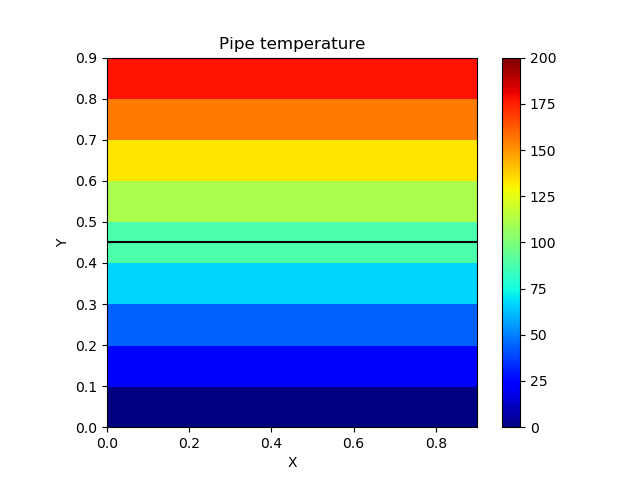
\includegraphics[width=0.5\linewidth]{temperature0.png} 
    % \includegraphics[width=0.5\linewidth, trim=0 250 0 250]{figures/cycle_tr_2.pdf} 
    \caption{\label{f:in0} Temperature of pipe for \texttt{input0.txt}. Mean temperature: 100.00002}
\end{figure}

\begin{figure}[h!]
    \centering
    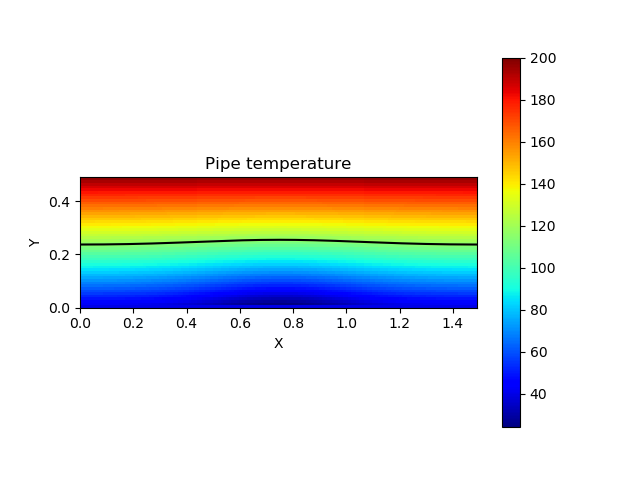
\includegraphics[width=0.7\linewidth]{temperature1.png} 
    % \includegraphics[width=0.5\linewidth, trim=0 250 0 250]{figures/cycle_tr_2.pdf} 
    \caption{\label{f:in1} Temperature of pipe for \texttt{input1.txt}. Mean temperature: 116.38993}
\end{figure}

\begin{figure}[h!]
    \centering
    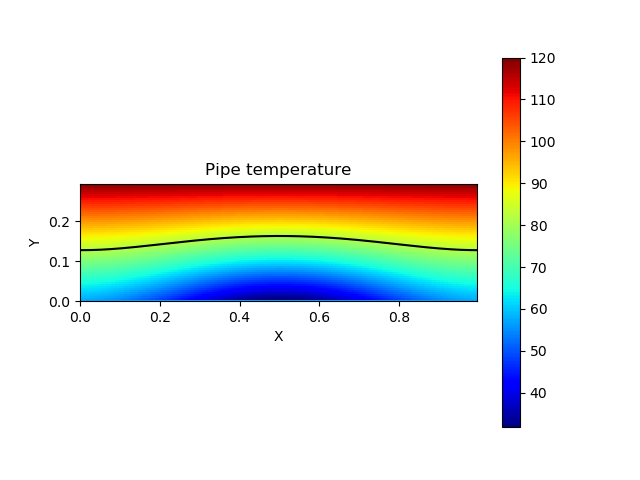
\includegraphics[width=0.7\linewidth]{temperature2.png} 
    % \includegraphics[width=0.5\linewidth, trim=0 250 0 250]{figures/cycle_tr_2.pdf} 
    \caption{\label{f:in2} Temperature of pipe for \texttt{input2.txt}Mean temperature: 81.99997}
\end{figure}

\end{document}
